% Adicionales
\begin{additional} 
\section{Capítulo Adicional que no es apéndice}
\end{additional}

% Apéndices
\begin{appendix} 
\section{Glosario}

\begin{enumerate}
\item{\textbf{PSF}}\\
\label{a1:psf}
Corresponde a la respuesta instrumental a una fuente de luz puntual, cuya radiaci\'on debe atravesar la atm\'osfera terrestre y los lentes del telescopio. La distorsi\'on puede ser interpretada como la convoluci\'on de la imagen por un kernel. \cite{huentelemu}. Ver imagen \ref{fig:a1}

\begin{figure}[h]
\centering
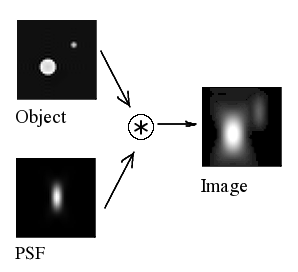
\includegraphics[scale=.5]{images/psf}
\caption{Ejemplo de distorsi\'on de una fuente al aplicar un kernel de PSF espec\'ifico. El resultado se observa en el cuado \textit{Image}.}
\label{fig:a1}
\end{figure}

\item{\textbf{Airmass}}\label{ap:airmass}\\
Es el largo del camino de que le toma a los rayos de una cuerpo celeste atravesar la atm\'osfera. A medida que los rayos van penetrando la atm\'osfera estos se van atenuando por la absorci\'on y el proceso conocido como scattering. 
\item{\textbf{Fotometr\'ia de Naylor}}\\
\end{enumerate}
\section{Refactoring}
\subsection{Librer\'ias usadas para el refactoring}
\label{subs:a0}
Versi\'on de Python: 3.5
\begin{itemize}
\item \textbf{\texttt{pandas}: 0.24.4}
\item \textbf{\texttt{matplotlib}: 2.2.2}
\item \textbf{\texttt{numpy}: 1.13.3}
\item \textbf{\texttt{mahotas}: 1.4.4}
\item \textbf{\texttt{astropy}: 3.0.2}
\end{itemize}
\subsection{Archivo de entrada: configuraci\'on de paths}
\label{subs:a1}
\VerbatimInput{/home/paloma/Documents/Memoria/Code/sif2/inputs/input_example.txt}
\section{Nueva funcionalidad}
\subsection{Modelo de archivo de almacenamiento de resultados}

\section{Unit-tests}
\subsection{Refactoring}
\begin{itemize}
\item \texttt{test\_input}\\
Comprueba que outputs generados de la lectura de los datos de la nueva versi\'on del programa sea identica a los generados por el c\'odigo original. Esto se logra siguiendo el proceso de filtrado de im\'agenes cient\'ificas por airmass con la consiguiente secuenciaci\'on cronol\'ogica (en t\'erminos de MJD) del resto de las im\'agenes.
\item \texttt{test\_flux}\\
Prueba el correcto funcionamiento de \texttt{calc\_flux} mediante comparaci\'on de outputs de versi\'on original y nueva.
\item \texttt{test\_basicKF}\\
Comprueba que las salidas de la versi\'on b\a'sica del filtro de Kalman del programa refactorizado sea id\'entico al de la versi\'on original, usando secuencia de im\'agenes conocida.
\item \texttt{test\_MCKF}\\
Comprueba que las salidas de la versi\'on de m\'axima correntro\'ia  del filtro de Kalman del programa refactorizado sea id\'entico al de la versi\'on original, usando secuencia de im\'agenes conocida.
\end{itemize}
\end{appendix}

